%%%%%%%%%%%%%%%%%%%%%%%%%%%%%%%%%%%%%%%%%%%%%%%%%%%%%%%%%%%%%%%%%%%%%%%%%%%
%% ws-rv9x6.tex   :   27 January 2003
%% Text file to use with ws-rv9x6.cls written in Latex2E.
%%
%% The content, structure, format and layout of this style file is the 
%% property of World Scientific Publishing Co. Pte. Ltd. 
%% Copyright 1995, 2002 by World Scientific Publishing Co. 
%% All rights are reserved.
%%
%% Review Volume Trim Size: 9in x 6in   (Without Content Text)
%% Text Area: 7.35in (include runningheads) x 4.5in
%% Main Text is 10/13pt					  
%%%%%%%%%%%%%%%%%%%%%%%%%%%%%%%%%%%%%%%%%%%%%%%%%%%%%%%%%%%%%%%%%%%%%%%%%%%

%\documentclass[draft]{ws-rv9x6}  
\documentclass{ws-rv9x6}  

\begin{document}

\setcounter{chapter}{0}

\chapter{DISSOCIATIVE ELECTRON--ION RECOMBINATION\\
STUDIES USING ION SYNCHROTRONS}

\markboth{M. Larsson}{Dissociative 
Electron--ion Recombination Studies using Ion Synchrotrons}

\author{Mats Larsson}

\address{Department of Physics, Stockholm University\\
P.O. Box 6730, S-113 85 Stockholm, Sweden\\
E-mail: mats.larsson\@physto.se}

\begin{abstract}
The abstract should summarize the context, content and conclusions of
the paper in less than 200 words. It should not contain any references
or displayed equations. Typeset the abstract in 9 pt Times roman with
baselineskip of 11 pt, making an indentation of 1.5 pica on the left
and right margins.
\end{abstract}

\section{Introduction}     %S1-Heads

Many chapters in this book deal with photoionization, which is a
process where an electron bound to an atom or molecule is transferred
to the electronic continuum by means of photon absorption. For an
atomic ion $A^{q+}$, radiative recombination of $A^{(q+1)+}$ can be
viewed as the inverse process of photoionization of $A^{q+}$. The free
electron attaches to $A^{(q+1)+}$ to form $A^{q+}$, and the excess
energy is carried away by a photon. If the ion $A^{(q+1)+}$ contains
bound electrons, the free electron can excite one of these electrons
while entering a bound atomic orbital. This is called dielectronic
capture and results in the formation of a doubly excited ion
[$A^{q+}$]$^{**}$, which is located in the ionization 
continuum of $A^{(q+1)+}$.

When a molecular ion captures an electron, the molecular analogues of
radiative and dielectronic recombination are in principle possible,
however, they are usually completely overshadowed by a process 
which is far more effective than any of the atomic processes
\begin{equation}	
A^{q+1} + A^{q+} \to A + B \,,
\end{equation}
where $A\in B=q+1$ and $B$ is in the radiative processes.

\begin{figure}[th]		%Fig~1
\centerline{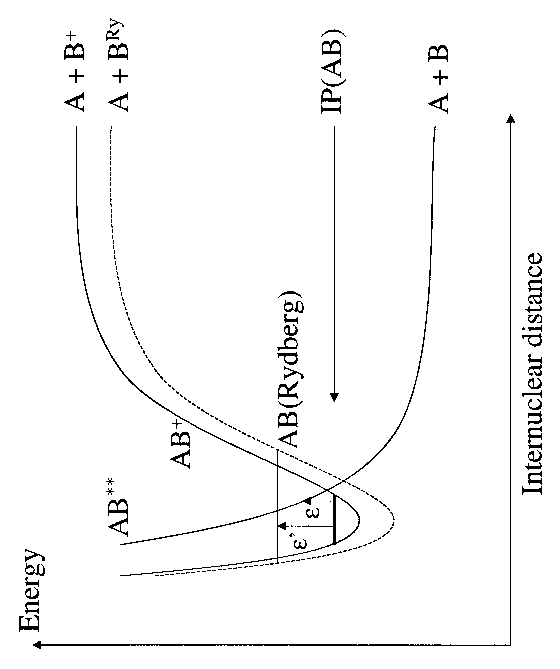
\psfig{file=rv-fig1.eps,width=2.6in,angle=-90}}
\vspace*{8pt}
\caption{A schematic illustration of dissociative recombination. The
direct mechanism is initiated when the molecular ion AB$^+$ captures
an electron with kinetic energy $\varepsilon$. The potential energy
function for the neutralized and electronically {\it doubly\/} excited
molecule AB$^{**}$ is strongly repulsive, which renders the two atoms
A and B to rapidly depart from each other. When the potential energy 
has dropped below the ionization potential, denoted IP(AB), the
electron capture process has been stabilized. The indirect mechanism
involves the capture of an electron with kinetic energy
$\varepsilon'$, so that a vibrationally and electronically {\it
singly\/} excited molecule AB(Rydberg) is formed. \label{fig1}}
\end{figure}

The reason for this process being so much more efficient than the
atomic processes is that a molecular ion can stabilize the capture of
an electron by making use of its internal structure, which allows for
a radiationless rearrangement of the nuclei on a time scale ($<1$~ps)
much shorter than that for radiative transitions ($>1$~ns).  
Figure~\ref{fig1} illustrates the process. The free electron can
deposit its excess energy to the molecular ion either by exciting a
bound electron or by exciting a vibrational mode. In order to prevent
autoionization,\index{autoionization} the molecule must lower its
electronic energy. This is achieved by rapid mole\-cular dissociation
along the repulsive potential energy curve of the doubly excited state
(the direct mechanism), hence the name ``dissociative
recombination''. If the free electron loses its energy by vibrationally
exciting the ion core, a radiationless transition (predissociation)
from the vibrationally excited Rydberg state to the repulsive doubly
excited state is required before dissociative stabilization of the
electron capture can occur (the indirect mechanism)\footnote{The paper
focuses on ASEAN because it is the only institutionalised regional
grouping in Asia. Yet, because of data availability the empirical
analysis is restricted to the five major- countries, namely Indonesia,
Malaysia, Philippines, Singapore and Thailand, while Brunei, Cambodia,
Laos Myanmar and Vietnam had to be excluded from the scope of the 
study.}. In contrast with the atomic case, the first step in the
direct mechanism, dielectronic capture, is not sharply resonant in the
molecular case.

Dissociative recombination involves radiationless transition(s) from a
molecular ion and a continuum electron to a nuclear continuum, and it
could involve a large number of Rydberg states. This renders the
process very difficult to treat theoretically. A further problem for
theoretical calculations is the sparsity of relevant molecular data.

A number of factors also conspire to make the process difficult to
study experimentally. Molecular ions are difficult to prepare and
maintain at high concentrations, and they are particularly difficult
to prepare with a well-defined vibrational distribution. The ions
should further be brought to interact with electrons with a {\it
known\/} velocity distribution. Depending on the experimental
technique, the production of neutral particles (beam techniques) or
the removal of charge (afterglow techniques, ion traps) is
monitored. In both cases there are other processes that give rise to
the same effect, and these processes can be corrected for.

The technique relying on the monitoring of neutral particles is based
on accelerated charged-particle beams. In order to have access to
very-low-energy collisions ($\sim1$~meV), the ion and electron beams
are merged at zero-degree angle over a known distance. Ion storage
rings represent the most recent advancement of the merged-beams
technique. In a storage ring, the molecular ions continuously
circulate at very high speed in an extremely high vacuum. The ions all
have nearly the same kinetic energy, and they occupy, for infrared
active modes, the lowest vibrational quantum level. This very clean
sample of ions serves as a well-defined target for a cold beam of
electrons which interact with the molecular ion beam over a distance
of about one meter. The application of ion storage ring technology to
the process of dissociative recombination, and related processes.

\section{History and Applications of 
Dissociative Recombination \label{seco2}}

The mechanisms of dissociative recombination are shown schematically
in the molecular ions. The direct mechanism was first suggested by
Bates.\cite{1} It is deceptively simple, but was long in coming, as
described in some detail in Bates' final article on the
subject.\cite{2} It was not until the microwave experiments by Biondi
and Brown\cite{3,4} that Bates was finally convinced that molecular
ions effectively recombines with electrons. The direct dissociative
recombination\index{direct dissociative recombination} cross-section
is inversely proportional to the electron energy, $\varepsilon$, and
proportional to the electronic which determines 
the process.

For dissociative recombination of polyatomic molecular ions it has so
far been possible in storage rings to measure only the branching
ratios into neutral products, but not their state of excitation. The
technique used for doing these measurements will be described in
Sec.~\ref{seco2}.

\section{Dissociative Recombination through a Crossing of Potential Curves}

The mechanism for dissociative recombination 
has been given the descriptive name the {\it crossing
mode}.\cite{2}\index{crossing mode} It was for a long time believed
that a favorable crossing was a prerequisite for the occurrence of
dissociative recombination. As we will see in the next section, a
second mode of recombination, the {\it tunneling
mode},\index{tunneling mode} has recently been recognized as
important. The recognition of this second mode came almost half a
century after Bates' seminal paper.\cite{1} Thus, it is natural that
the majority of molecular ions for which theoretical and experimental
dissociative recombination data are available belongs to the crossing
mode category.

\begin{table}		%Table~1.
\tbl{Calculated $r$-mode frequency corrections $\omega_2$ for constant
density stars ($n=0$) and $n=1$ polytropes. Results are shown both for
the full calculation (nC) and the Cowling approximation (C). The
results are for barotropic perturbations and the fundamental $l=m$
modes.} 
{\tabcolsep10pt
\begin{tabular}{@{}c@{\hspace*{0.7cm}}cc@{}c@{\hspace*{0.25cm}}cc@{}}
\hline\\[-7pt]
& \multicolumn{2}{@{}c@{}}{$\omega_2(n=0)$} 
& \hspace*{0.5cm} & \multicolumn{2}{@{}c@{}}{$\omega_2(n=1)$} \\[3pt]
\cline{2-3} 
\cline{5-6}\\[-7.2pt]
& nC & C & & nC & C \\[3pt]
\hline\\[-7.2pt]
2 & 0.765 & 0.913 & & 0.398 & 0.451 \\
3 & 0.777 & 0.844 & & 0.527 & 0.423 \\
4 & 0.769 & 0.345 & & 0.656 & 0.382 \\
5 & 0.730 & 0.749 & & 0.399 & 0.405 \\[3pt]
\hline
\end{tabular}} 
\label{table1}
\end{table}

Table~\ref{table1} lists all ion storage ring experiments known to the author
concening dissociative recombination that have resulted in a published
paper, a paper that is in press, or a paper that has been submitted
for publication (by August 1998), and the type of results that have
been obtained in these experiments. Examples of the theoretically
computed Doppler spectra.  (Thick line: $0^\circ$ crossing angle, thin
line: $90^\circ$ crossing angle). The results of the 
present model depend importantly on our assumption 
that the spectra retains a long-term interest.

\subsection{Diatomic Hydrogen Ions}

Being the simplest diatomic molecule, it is natural that H$_2^+$ and
its isotopomers represent benchmark systems for dissociative
recombination, in particular with respect to the comparison of
experiment and theory. The experimental and theoretical studies of DR
of H$_2^+$ and its isotopomers in their zeroth vibrational levels are
described in some detail in two recent reviews,\cite{2,32} and only a
brief summary of the present situation will be given here.

The development of a single-pass merged electron-molecular ion beams
technique\cite{65} played an important role for the understanding of
DR of H$_2^+$. Because of the rapid conversion of H$_2^+$ to H$_3^+$
by ion--molecule reactions, H$_2^+$ is inaccessible to the afterglow
techniques. The merged beams (see Table~\ref{table2}) 
technique\index{merged beams technique}
also allows the measurement of DR cross-sections or 
early experimental and theoretical papers\cite{6,7} provided the
first qualitatively correct insight into the DR of H$_2^+$, it was not
until more than ten years later that a complete quantitative
comparison of experiment and theory finally was accomplished by the
research groups of Giusti-Suzor and Mitchell.\cite{66}\cdash\cite{69}
The comparison revealed a good agreement both in terms of the absolute
values of the cross-section and the positions of several `window'
resonances caused by the interference between the direct and indirect
mechanisms.

\begin{table}[th]      %Table~2
\def\p{\phantom{0000}}
\tbl{Predicted and observed order of errors for eigenvalues based on
various combinations of stiffness and mass matrices.\label{table2}}
{\begin{tabular}{@{}cccccc@{}}
\toprule
Type &\multicolumn{3}{c}{Predicted order of error in representing} 
&{} &Observed error for\\[0.8ex]
\cline{2-4} \cline{6-6}\\[-2ex]
{} &$K$ &\phantom{000}$M$ &$\lambda$ &{} &$\lambda$\\
\colrule
k2r--m2c &$O(h^2)$ &\p$O(h^4)$ &$O(h^2)$ &{}
&$O(h^2)$\\[0.4ex]
k2r--m2l &$O(h^2)$ &\p$O(h^2)$ &$O(h^2)$ &{} &$O(h^2)$\\[0.4ex]
k3e--m3c &$O(h^2)$ &\p$O(h^6)$ &$O(h^2)$ &{} &$O(h^2)$\\[0.4ex]
k3e--m3l &$O(h^2)$ &\p$O(h^4)$ &$O(h^2)$ &{} &$O(h^2)$\\[0.4ex]
k3r--m3a &$O(h^4)$ &\p$O(h^6)$ &$O(h^3)$ &{} &$O(h^3)$\\[0.4ex]
k3e--m3b &$O(h^5)$ &\p$O(h^7)$ &$O(h^4)$ &{} &$O(h^7)$\\[0.4ex]
k3r--m3d &$O(h^7)$ &\p$O(h^8)$ &$O(h^6)$ &{} &$O(h^8)$\\
\botrule
\end{tabular}}
\begin{tabnote}[Note$:$]
The rapid conversion of $O(h^2)$ to $O(h^4)$ by ion--molecule reactions.
\end{tabnote}
\begin{tabnote}[Source$:$]
Takagi (1996).
\end{tabnote}
\end{table}

The comparison concerned only DR at electron energies well
below the ion dissociation energy, where the 
$(2p \sigma_u)^2\, ^1 \Sigma_g^+$ resonant state 
completely dominates the recombination. It was not possible, 
however, to unambiguously assign the experimental results to
H$_2^+$ populating only its zeroth vibrational level of the molecule.

\begin{sidewaystable}	%Table~3
\tbl{Sample statistics for A-share premia for Shanghai companies that 
issued A- and B-shares before April 1994 (sample period: April 1, 
1994--October 31, 1998). \label{table3}}
{\begin{tabular}{@{}ccccccccc@{}}
\hline
\multicolumn{9}{c}{}\\[-2ex]
Year &Taiwan &Dow Jones &Nikkei &South &London's &Hong Seng &Thailand's
&Singapore's\\
{} &Index &Index &Index &Korea's &FTSE &Index &Set Index &Strait Times\\
{} &{} &{} &{} &Kospi &Index &{} &{} &{}\\
{} &{} &{} &{} &Index &{} &{} &{} &{}\\[0.25ex]
\hline
\multicolumn{9}{c}{}\\[-2ex]
1988 &5,119.11 &\phantom{0}2,168.57 &30,159.00 &907.20 &1,455.30
&\phantom{0}2,687.44 &386.73 &1,038.62\\ 
1989 &9,624.18 &\phantom{0}2,753.20 &38,915.87 &909.72 &1,916.60
&\phantom{0}2,836.57 &879.19 &1,481.33\\
1990 &4,530.16 &\phantom{0}2,633.70 &23,848.71 &696.11 &1,673.40
&\phantom{0}3,243.30 &612.86 &1,154.48\\
1991 &4,600.67 &\phantom{0}3,168.83 &22,983.77 &610.92 &1,891.30
&\phantom{0}4,297.33 &711.36 &1,490.70\\
1992 &3,377.06 &\phantom{0}3,301.11 &16,924.95 &678.44 &2,185.20
&\phantom{0}5,512.39 &893.42 &1,524.40\\
1993 &6,070.56 &\phantom{0}3,754.09 &17,417.24 &866.18 &2,559.50
&11,888.39 &1,565.12\phantom{0.} &2,425.68\\
1994 &7,124.66 &\phantom{0}3,834.44 &19,723.06 &1,027.37\phantom{0.}
&3,065.50 &\phantom{0}8,191.04 &1,360.09\phantom{0.} &2,239.56\\
1995 &5,173.73 &\phantom{0}5,117.12 &19,868.15 &882.94 &3,689.30
&10,073.39 &1,280.81\phantom{0.} &2,266.54\\
1996 &6,933.94 &\phantom{0}6,448.27 &19,361.35 &651.22 &4,118.50
&13,451.45 &831.57 &2,216.79\\
1997 &8,187.27 &\phantom{0}7,905.25 &15,258.74 &376.31 &5,135.50
&10,722.76 &372.69 &1,529.84\\
1998 &6,418.43 &\phantom{0}9,181.43 &13,842.17 &562.46 &5,882.60
&10,048.58 &355.81 &1,392.73\\
1999 &8,448.84 &11,497.12 &18,934.34 &1,028.07\phantom{0.} &6,930.20
&16,962.10 &481.92 &2,479.58\\
2000 &5,544.18 &10,971.14 &14,539.60 &514.48 &6,438.40 &14,895.34
&271.84 &1,976.54\\ 
1 &9,744.89 &10,940.53 &19,539.70 &943.88 &6,268.50 &15,532.34 &477.57
&2,230.28\\
2 &9,435.94 &10,128.31 &19,959.52 &828.38 &6,232.60 &17,169.44 &374.32
&2,120.50\\
3 &9,854.95 &10,921.92 &20,337.32 &860.94 &6,540.20 &17,406.54 &400.32
&2,132.59\\
4 &8,777.35 &10,733.91 &17,973.70 &725.39 &6,327.40 &15,519.30 &390.40
&2,164.11\\
5 &8,939.52 &10,522.33 &16,332.45 &731.88 &6,359.30 &14,713.86 &323.29
&1,795.13\\
6 &8,265.09 &10,447.89 &17,411.05 &821.22 &6,312.70 &16,155.78 &325.69
&2,037.97\\
7 &8,114.92 &10,521.98 &15,727.49 &705.97 &6,365.30 &16,840.98 &284.67
&2,051.21\\
%8 &7,616.98 &11,215.10 &16,861.26 &688.62 &6,672.70 &17,097.51 &307.83
%&2,147.77\\[0.5ex]
\hline
\end{tabular}}
\begin{tabnote}
The state-budget funds as a dominant financial source of investment 
of SOEs, regardless of investment decisions being made by governments 
or enterprises. The retained profits and non-bank debts are also used by
SOEs to finance their investment and operation.
\end{tabnote}
\end{sidewaystable}

\begin{sidewaystable}	%Table4
\tbl{Abnormal returns and firm characteristics 
for equity issues.\label{table4} \vspace*{-6pt}}
{\begin{tabular}{@{}lcccccccc@{}}  
\toprule
& \multicolumn{2}{c}{Stock dividend} & \multicolumn{2}{c}{Rights
offers} &\multicolumn{2}{c}{Divd. \& rights}
&\multicolumn{2}{c}{Underwritten} \\[2pt] 
\cline{2-9} 
& &  &  &  & &  &  &  \\ [-5pt] 
& Mean & Median & Mean & Median & Mean & Median & Mean & Median \\ [2pt] 
\colrule
ADAR & -1.47\% & -0.92\% & 7.04\% & 2.82\% & -9.08\% & -1.08\% &
-0.43\% & -0.70\% \\ [3pt] 
CASHTA & 0.0832 & 0.0636 & 0.0945 &
0.0634 & 0.0953 & 0.0804 & 0.1057 & 0.0872 \\ [3pt] 
LIQUIDTA &
0.5590 & 0.5627 & 0.5683 & 0.5762 & 0.5524 & 0.5306 & 0.5581 &
0.5740 \\ [3pt] 
LEVERAGE & 0.0563 & 0.0214 & 0.0304 & 0.0122 &
0.0579 & 0.0362 & 0.0633 & 0.0248 \\ [3pt] 
MVE & 577.87 & 124.54
& 957.95 & 347.56 & 298.88 & 115.63 & 469.31 & 205.58 \\ [3pt]
MKTBOOK & 1.1973 & 1.0244 & 1.5584 & 1.2493 & 1.2054 & 1.1351 &
1.4188 & 1.1297  \\ [3pt] 
LONGINV & 0.1193 & 0.0804 & 0.1525 &
0.1142 & 0.1077 & 0.0757 & 0.1458 & 0.1083 \\ [3pt] 
PROFSHA &
0.0228 & 0.03251 & 0.1625 & 0.1843 & 0.0477 & 0.0543 & 0.0486 &
0.0528 \\ [3pt] 
CAR-120 & -14.04\% & -15.34\% & 6.53\% & 4.42\%
& -16.6\% & -16.71\% & 2.54\% & 2.33\% \\ [3pt] 
CAR+120 & -5.01\% & -4.40\% & 12.04\% & 13.68\% & -5.73\% & -6.71\% &
-1.48\% & -2.25\% \\ [3pt] 
CAR+360 & -6.13\% & -5.89\% & 6.97\%
& 8.08\% & -7.13\% & -7.28\% & 2.06\% & 3.14\%  \\ [3pt] 
BETA &
1.5227 & 1.6080 & 1.3108 & 1.3295 & 1.4762 & 1.4536 & 1.4419 &
1.5239 \\ [3pt] 
STD & 4.93\% & 3.90\% & 3.74\% & 3.58\% & 5.09\%
& 4.15\% & 4.37\% & 4.02\% \\ [3pt] 
GOVNT & 24.31\% & 21.50\% &
16.67\% & 14.55\% &  18.53\% & 15.69\% & 8.26\% & 7.73\% \\ [3pt]
TOPTEN & 72.08\% & 70.40\% & 54.07\% & 52.16\% & 86.46\% &
85.92\% & 63.94\% & 60.05\% \\ [3pt] 
MGOWN & 0.24\% & 0.22\% &
0.73\% & 0.68\% & 0.09\% & 0.09\% & 0.55\% & 0.54\% \\ [3pt]
\botrule
\end{tabular}}
\begin{tabnote}[Note$:$]  
The quota is distributed to individual provinces and then to
individual firms.  When a firm is approved for a listing, it usually
sets an IPO price so that the price-earning ratio is around 15 to 25.
To issue foreign shares, firms must obtain special approval from the
CSRC and local security regulatory authorities.
\end{tabnote}
\end{sidewaystable}

\subsection{Monohydride Ions}

Dissociative recombination of monohydride ions has been reviewed\break
recently.\cite{2,32} The process which involves an electronic
excitation of the ionic core has not been further investigated since
the last review.\cite{32} An imaging experiment with OH$^+$ in CRYRING
led to discovery of a very small kinetic energy release when the
electron energy was sufficient for the ${\rm O}(^3P) + {\rm H}(n=2)$
dissociation limit (see Table~\ref{table3}) to become energetically
allowed.\cite{84} Recombination of OH$^+$ is known to proceed through
the 2 $^2\Pi$ resonant state,\cite{85} which dissociates diabatically
to ${\rm O}(^1D) + {\rm H}(n=1)$. The imaging result (see
Table~\ref{table4}) shows that part of the dissociating flux is
redirected, probably at avoided crossings between the 2 $^2\Pi$ state
and the 3 $^2\Pi$, 4 $^2\Pi$ and 5 $^2\Pi$ states, which all correlate
diabatically to the ${\rm O}(^3P) + {\rm H}(n=2)$ limit. It is thus
reasonable to approximate the actual pressure with its time average
over one period (that is, set $p=0$) provided the radius $R$.

These are generally accepted as the yardstick for determining whether
or not a method qualifies as being intelligent. Neural-networks,
genetic algorithms, tabu search, and ant systems are presented as
being adaptive memory programming.

\subsection{Nonhydride Diatomic Ions}

This category is dominated by the three atmospherically important ions
O$_2^+$, N$_2^+$, and NO$^+$, but also CO$^+$ and CN$^+$ will be
discussed.

The parameter estimates using Generalized Least Squares (GLS). As
shown in the table, $\hat{\delta}_1$ is significantly positive at the
5\% level, suggesting that A-share market beta is a good measure of
risk for an individual firm's share. It is not a question simply of
tracing funds but, rather, of assigning property rights. The competing
claimants various government departments and agencies often cannot
reach consensus on who the investor is.

The solution of the ICAPM also clearly shows that cross-sectional
variations in the expected return between domestic and foreign shares
are determined by the shares' own market betas and betas with respect
to the international financial markets.  Given that we reach the same
results using two different theoretical models, we firmly believe that
we have solid ground for further empirical work. 

It shows changes in proportions of the central
government's projects and local projects in the total capital
construction investment of state-owned sector. Investment decisions of
central projects are generally made by the line ministries and the
State Planning Commision, and that of local projects, 
(see Table~\ref{table5}) are made by local governments and enterprises. 

\begin{center}
\begin{table}	%Table~5		
\tbl{Probability of strength modification.}
{\begin{tabular}{@{}lcccc@{}}
\cline{1-5}
\raisebox{0pt}[10pt][0pt]{Probability of}
& \raisebox{0pt}[10pt][0pt]{$\phi$} 
& \raisebox{0pt}[10pt][0pt]{$\phi$}
& \raisebox{0pt}[10pt][0pt]{$\gamma$} 
& \raisebox{0pt}[10pt][0pt]{$\gamma$}\\[-0.2ex] 
\raisebox{0pt}[8pt][0pt]{nonexceedance}
& \raisebox{0pt}[8pt][0pt]{for Column} 
& \raisebox{0pt}[8pt][0pt]{for Beam} 
& \raisebox{0pt}[8pt][0pt]{for Column}
& \raisebox{0pt}[8pt][0pt]{for Beam}\\[0.6ex]
\hline
\raisebox{0pt}[10pt][0pt]{90\%}
& \raisebox{0pt}[10pt][0pt]{1.01} 
& \raisebox{0pt}[10pt][0pt]{0.97} 
& \raisebox{0pt}[10pt][0pt]{1.49}
& \raisebox{0pt}[10pt][0pt]{1.11}\\
\raisebox{0pt}[10pt][0pt]{95\%} 
& \raisebox{0pt}[10pt][0pt]{0.94} 
& \raisebox{0pt}[10pt][0pt]{0.95}
& \raisebox{0pt}[10pt][0pt]{1.55}
& \raisebox{0pt}[10pt][0pt]{1.13}\\
\raisebox{0pt}[10pt][0pt]{99.9\%}
& \raisebox{0pt}[10pt][0pt]{0.67}
& \raisebox{0pt}[10pt][0pt]{0.88}
& \raisebox{0pt}[10pt][0pt]{1.83}
& \raisebox{0pt}[10pt][0pt]{1.20}\\[0.6ex]
\hline
\multicolumn{4}{l}{\kern-5.6pt\raisebox{0pt}[10pt][0pt]{$\psi$: strength
modification factor for dependable strength.}}\\
\multicolumn{4}{l}{\kern-5.6pt\raisebox{0pt}[0pt][0pt]{$\gamma$: strength
modification factor for upper bound strength.}}\\[-5ex]
\end{tabular}}
\label{table5}
\end{table}
\end{center}

\subsubsection{Transition in the Theoretical Work}

The thermal rate coefficient for O$_2^+$ occupies an unusual role in
the respect that different experiments over a time span of thirty
years almost unanimously agree\cite{2} that $\alpha$(O$_2^+$) $\approx
2 \times 10^{-7}$~cm$^3$s$^{-1}$, the very recent measurement based on
cross-section data from CRYRING being no exception.\cite{86} With few
exceptions,\cite{87} most theoretical work has been devoted to the
understanding of the formation of O($^1S$) in dissociative 
recombination of O$_2^+$. It is the O($^1S$) $\to$ O($^1D$) transition
in neutral atomic oxygen which gives rise to the green
airglow\index{green airglow} at 5577~\AA\ in the terrestrial
atmosphere. It is worth noting that the earliest mention of
dissociative recombination was made in an attempt to identify a source
of the green oxygen line.\cite{88}
Guberman showed\cite{89,90} that DR of O$_2^+ (\nu < 10)$ leading to
the production of ${\rm O}(^1S)$ must occur through the $^1
\Sigma_u^+$ state of O$_2$ that dissociates to ${\rm O}(^1S) + {\rm
O}(^1D)$, and proceeded to calculate, using the MQDT approach,
the partial rate coefficient for DR of O$_2^+$ through the $^1 \Sigma_u^+$
state.\cite{91} 

\section*{Examples of Listings and Theorem Environments}

\subsection*{Test for Lists}

\begin{itemlist}
 \item item one,
 \item item two,
\item item three.
\end{itemlist}
Items may also be numbered in lowercase roman numerals:
\begin{romanlist}
\item item one
\item item two
\item item three
	\begin{romanlist}[(b)]
	\item Lists within lists can be numbered with lowercase 
              roman letters,
	\item second item. 
	\end{romanlist}
\end{romanlist}

\subsection*{Test for Theorem Environments}

\begin{theorem} \label{th1}
In any unital Banach algebra $A,$ the spectrum of each $a\in A$ is a
non-empty compact subset, and the resolvent 
function is analytic on ${\bf C} \setminus {\rm sp}(a).$
\end{theorem}

We see that the crucial assumption of the mechanism is that despite
the vanishing of the bare fermion mass, the physical mass $m$ of the
fermion is nonzero. Since the bare fermion mass $m_0=0$, we have
$A={\bf C}$, see Theorem~\ref{th1} and so we obtain the 
self-consistency equation for the physical mass of fermion.

\begin{proof}
On ${\mathbb Y}\setminus (A\times {\mathbb P}^1)$, $p$ is just 
$h$ and its singularities are isolated. The notation $A$ stays for 
$\hat A\cap Y$.
\end{proof}

The first statement immediately follows from the definition of the
spaces $\mathbb Y$ and $\mathbb X$. As for the second statement, we
have the homotopy equivalences
\begin{equation}	
\pi_{i +1} (Y)\simeq \pi_i (Y_S, X_\alpha)\,.
\label{eq:1}
\end{equation}
We need a condition which implies a certain level of connectivity of
each pair $(B_i\cap {\mathbb Y}_D, B_i\cap {\mathbb X}_c)$. A
condition that fits well is the rectified homotopical depth of the
total space $\mathbb X$. This condition does not depend on the
stratification of the space.

Moreover,
\begin{equation}\label{I1e1}
\lim_{|\lambda|\to\infty}\|R(\lambda)\|\le \lim_{|\lambda|\to\infty}
\frac{|\lambda|^{-1}}{1-( \frac{\|a\|}{\lambda})}=0\,.
\end{equation}
Similarly, 
if $\lambda_0-a$ is invertible and 
$|\lambda-\lambda_0| < \frac{1}{\|(\lambda_0-a)^{-1}\|} ,$ then 
\[
(\lambda-a)^{-1}=\sum_{n=0}^{\infty} (\lambda_0-\lambda)^n 
((\lambda_0-a)^{-1})^{n+1}\,.
\]
This also shows that the resolvent is open.  Since ${\rm sp}(a)$ has
been shown to be bounded, ${\rm sp}(a)$ is compact.  We have also
shown that the resolvent function is analytic on the complement of the
spectrum.

\begin{definition}\label{I1Da1}
A Banach algebra $A$ is said to be {\it
unital}\index{algebra!Banach!unital} if it admits a unit $1$ and
$\|1\|=1.$ Banach algebras in \ref{I1e1}.
\end{definition}

\begin{lemma}\label{I1L1}
Let $A$ be a unital Banach algebra and $a$ be an element
of $A$ such that $\|1-a\|<1.$ Then $a\in GL(A)$ and 
\[
a^{-1}=\sum_{n=0}^{\infty}(1-a)^n\,.
\]
Moreover, $\|a^{-1}\| \le \frac{1}{1-\|1-a\|}$ 
and $\|1-a^{-1}\|\le \frac{\|1-a\|}{1-\|1-a\|}.$
\end{lemma}

\begin{remark}\label{I2RC}
{\rm The Gelfand representation theorem for commutative $C^*$-algebras
is fundamentally important. Even in a non-commutative $A$ we often
obtain useful information of $A$ via the study of certain commutative
$C^*$-subalgebras of $A$. So Theorem~\ref{th1} certainly plays an important role
in studying non-commutative $C^*$-algebras as well.  Theorem 2 shows
that to study commutative $C^*$-algebras, it is equivalent to study
their maximal ideal spaces.  So the commutative $C^*$-algebra, theory
is the theory of topology. Much of general $C^*$-algebra, theory can
be described as non-commutative topology.}
\end{remark}

\begin{corollary}\label{I1C1}
The only simple commutative unital Banach algebra is ${\bf C}.$
\end{corollary}

\begin{proof}
Suppose that $A$ is a unital commutative Banach algebra and 
$a\in A$ is not a scalar. Let $\lambda\in {\rm sp}(a).$
Set $I={\overline{(a-\lambda)A}}.$ Then $I$ is clearly
a closed ideal of $A.$ No element of the form 
$(a-\lambda)b$ is invertible in the commutative Banach algebra
$A.$ By \ref{I1L1}, 
\[
\|(a-\lambda)b-1\|\ge 1\,.
\]
So $1\not\in I$ and $I$ is proper. Therefore, if $A$ is simple, 
$a$ must be a scalar, whence $A={\bf C}.$
\end{proof}

\begin{example}
Let $X$ be a compact Hausdorff space and 
$C(X)$ the set of continuous functions on $X.$
$C(X)$ is a complex algebra with pointwise operations.
With $\|f\|=\sup_{x\in X}|f(x)|,$ $C(X)$ is a 
Banach algebra.
\end{example}

\begin{proposition}
Let $B$ be a $C^*$-subalgebra of a $C^*$-algebra and $A$. For 
each positive linear functional $\phi$ on $B$ there is a positive 
linear functional ${\tilde \phi}$ on $A$ such that 
${\tilde \phi}|_B=\phi$ and $\|{\tilde \phi}\|=\|\phi\|.$  
If furthermore $B$ is hereditary, then the extension is unique.
\end{proposition}

\begin{example}
Let $M_n$ be the algebra of $n\times n$ complex matrices. By
identifying $M_n$ with $B({\bf C}^n),$ the set of all (bounded) linear
maps from the $n$-dimensional Hilbert space ${\bf C}^n$ to ${\bf
C}^n,$ with operator norm, i.e, $\|x\|=\sup_{\xi\in {\bf C}^n,
\|\xi\|\le 1}\|x(\xi)\|, $ we see that $M_n$ is a Banach algebra.
\end{example}

\section{Tunneling Dissociative Recombination}

Convinced by overwhelming experimental evidence that HCO$^+$
recombines with a rate coefficient larger than
$10^{-7}$~cm$^3$s$^{-1}$, and by theoretical predictions that its
electronic ground state does not possess a favorable neutral state
crossing, Bates introduced a multistep indirect mechanism which does
not require a curve crossing.\cite{97} He later gave this mechanism
the decriptive name `tunneling dissociative recombination'.\cite{2}

\begin{figure}[th]		%Fig~2
\centerline{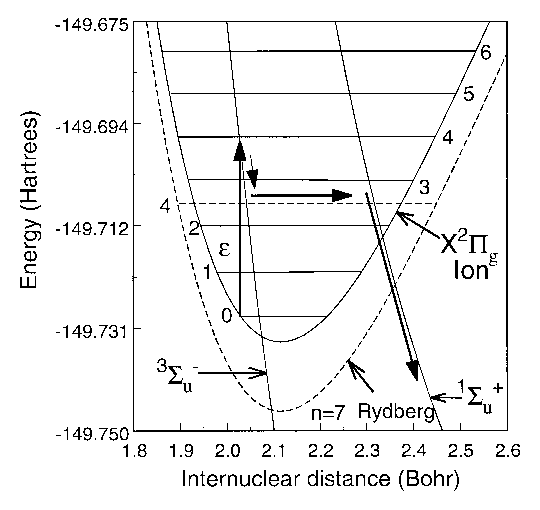
\psfig{file=rv-fig2.eps,width=3in}}
\vspace*{8pt}
\caption{Potential energy curves for O$_2^+$ and O$_2$. \label{fig2}}
\end{figure}

Figure~\ref{fig2} shows the relevant potential curves of O$_2^+$ and
O$_2$. The $^1 \Sigma_u^+$ state crosses the ion ground state close to
the right turning point of $\nu=2$. It is immediately obvious from the
potential curves that $\nu=0$ is expected to have a much lower quantum
yield than are $\nu=1$ and 2 (neglecting for a moment the new
mechanism shown in Fig.~\ref{fig2}).

The aim of the present notes is to allow the variable $R$ to have
quantum fluctuations around the classical trajectory and modify the
expressions of the general formalism.  Of course, it would be much
more interesting to allow for inhomogeneous fluctuations, but this
would inevitably render the system intractable analitically and is
left for future developments.

\begin{sidewaysfigure}		%Figure3
\centerline{\psfig{file=rv-fig3.eps,width=14cm}}
\caption{Change in pattern of financial sources of  
fixed shares investment. Time-series differences in average weekly 
returns between B and A shares.\label{fig3}} 
\end{sidewaysfigure}

\begin{sidewaysfigure}		%Figure4
\centerline{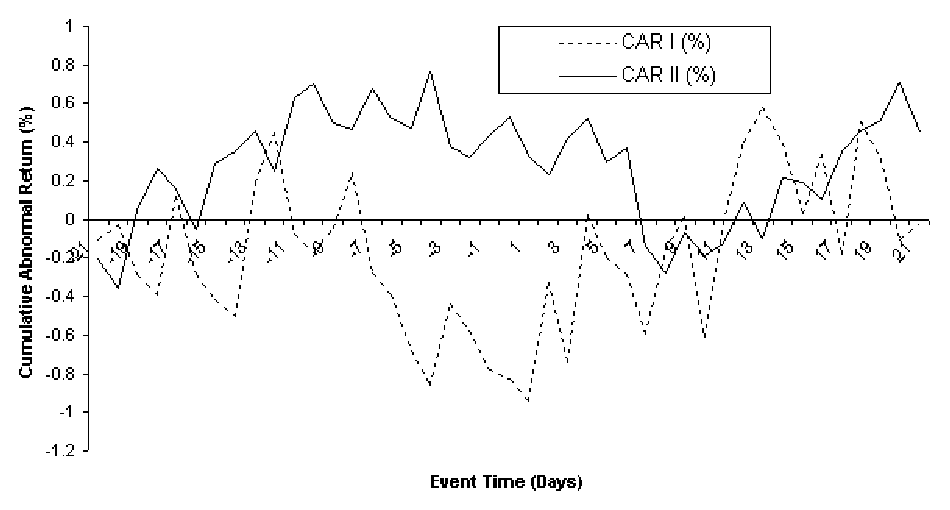
\psfig{file=rv-fig4.eps,width=16cm}}
\caption{The aggregate demand for car models. \label{fig4}} 
\end{sidewaysfigure}

\subsection{HeH$^{+}$}

The FALP measurement\cite{38} of a thermal rate coefficient less than 
$1 \times 10^{-10}$~m$^3$ for HeH$^+$ was seemingly in
perfect harmony with the absence of a curve crossing. The sizeable
cross-section measured in a merged beams experiment therefore
came as a surprise. The findings inspired theoretical
work,\cite{40,41} which finally identified coupling by the nuclear
kinetic-energy\break
operator of the HeH$^+$ ground state to close lying
(but not crossing) Rydberg states of HeH as the driving mechanism.

Let $S_j$ be such a close neighbor\index{close neighbor} and
${\mathcal L} (S_j)$ be the local packing of $S_j$ contained in
${\mathcal L}^2 (S)$. Then ${\mathcal L} (S_j) \cap {\mathcal L} (S)$
already constitutes a {\it partial\/} local packing of $S_j$ while the
others of ${\mathcal L} (S_j)$ are exactly those additional neighbors
belonging to the second layer of ${\mathcal L}^2 (S)$. Thus, the {\it
restriction\/} of the extension (see Fig.~\ref{fig3}), 
${\mathcal L} (S) \subset {\mathcal L}^2 (S)$, 
to that of ${\mathcal L} (S_j)$ is an extension from the 
partial one, ${\mathcal L} (S_j) \cap {\mathcal L} (S)$, to a
full-fledged local packing.

Herbst and Lee\cite{21} have found from model calculations on dark
interstellar clouds (see Fig.~\ref{fig4}) that although the breakup into
neutral reaction products in DR of polyatomic ions is more substantial
than previously believed, a general branching fraction of 0.30 for the
single H atom channel is still sufficient to give molecular abundances
in excellent agreement with observations. However, if this branching
fraction is lowered to 0.05, a larger change in predicted abundances
occurs. Such low branching was indeed measured for CH$_5^+$, but so
far this is the exception rather than the rule, at least as far as the
storage ring results are concerned.

\section{Conclusions and Outlook}

This article has focussed almost exclusively on the use of ion
storage rings for the study of dissociative recombination of
positively charged molecular ions with electrons. It is pertinent at
this point to recall that ion storage rings by no means are confined
to the study of this particular molecular process. Dissociative
excitation has already been mentioned in passing, with a reference
given to a recent review of the topic.\cite{33} But there are also
other aspects of molecular physics that can be addressed by means of
the storage ring technology, as discussed in a recent article by
Zajfman,\cite{22} and as witnessed by publications on electron impact
detachment of negative molecular ions,\cite{23,24} laser 
photodetachment spectroscopy of fullerenes,\cite{25} 
and laser photofragment spectroscopy.\cite{26}

Dissociative recombination of the simplest ion, H$_2^+$ and its
isotopomers, is beginning to be well understood. Yet, discrepancies
between experiment and theory still remain. They will most probably be
cleared up within the next couple of years. A good understanding of DR
of HeH$^+$ is also emerging, although there are still large
discrepancies between experiment and theory for some of the
isotopomers. 

The importance of HeH$^+$ lies in fact that it is the simplest is to
recombine the (tunneling mode). The primary actors of the modern
corporation are shareholders, the board of directors, and managers.
These three entities can be found in companies in developed countries,
although variant forms of organization exist in some countries.
Shareholders have all the rights related to property rights.

\section*{Acknowledgments}
\addcontentsline{toc}{section}{Acknowledgements}

This work was supported by the Swedish Natural Science Research
Council, the G\"oran Gustafsson Foundation, and by the Human Capital
and Mobility programme of EU. I would like to thank those who provided
preprints or unpublished material that was used in this article, and
A. Suzor-Weiner, G. H. Dunn, and W. Shi for valuable comments on the
early drafts.

\appendix

\section{First Appendix}

\renewcommand{\theequation}{A.\arabic{equation}}

Appendices should be used only when absolutely necessary. They
should come before the References. If there is more than one
appendix, number them alphabetically. Number displayed equations
occurring in the Appendix in this way, e.g.~(\ref{appen1}), (A.2),
etc.
\begin{equation}
\mu(n, t) = {\sum^\infty_{i=1} 1(d_i < t, N(d_i) = n) \over
\int^t_{\sigma=0} 1(N(\sigma) = n)d\sigma}\,. \label{appen1}
\end{equation}

\section{Second Appendix}

\renewcommand{\theequation}{B.\arabic{equation}}

References in the text are to be numbered consecutively in Arabic
numerals,\break
\eject

\noindent
in the order of first appearance. They are to be typed in 
superscripts after punctuation marks, e.g.

(1) $ \qquad $ ``$\ldots$ in the statement.\cite{6}''

(2) $ \qquad $ ``$\ldots$ have proven\cite{6} 
that this equation $\ldots$''

\noindent
This is done using the command: ``$\backslash$cite\{name\}''. 

When the reference forms part of the sentence it should not 
be superscripts, e.g.

(1) $ \qquad $  ``One can deduce from Ref.~\refcite{2} that $\ldots$''

(2) $ \qquad $  ``See Refs.~\refcite{1}--\refcite{3}, \refcite{4} 
and \refcite{6} for more details.'' 

(3) $ \qquad $  ``We refer the readers to Ref.~\refcite{6}.''

\noindent
This is done using the command: ``Ref.$\sim$$\backslash$refcite\{name\}''.

\vspace*{8pt}
\noindent
(Alternatively you may opt to use the default square bracket [\ ] 
citation throughout.)

\section{Footnotes}
Footnotes should be numbered sequentially in superscript lowercase
roman letters.\footnote{Footnotes should be typeset in 8~pt Times
roman at the bottom of the page.}

\section{Standard Abbreviations}
\begin{alphlist}[(d)]
\item Do not abbreviate the first word of any sentence: 

$ \qquad $ ``Figure~2 shows us $\ldots.$''

\item Some abbreviation:

$ \qquad $ ` figure ' $ \, $ = $ \, $  ` Fig. '

$ \qquad $ ` figures ' $ \, $ = $ \, $ ` Figs. '

$ \qquad $ ` equation ' $ \, $ = $ \, $ ` Eq. '

$ \qquad $ ` equations ' $ \, $ = $ \, $ ` Eqs. '

$ \qquad $ ` Section~5 ' $ \, $ = $ \, $ ` Sec.~5 '

$ \qquad $ ` Sections~5 and 6 ' $ \, $ = $ \, $ ` Secs.~5 and 6 '

$ \qquad $ ` for example ' = ` e.g. '

\noindent
Note that the first letter is capitalized. There is also a dot. 

\item When it is not appropriate, DO NOT abbreviate. Hence the word `Table'
is not abbreviated. We also do not write `Eq. of motion'.

\item Depends on authors' preference, sometimes ` Eq. ' and ` Eqs. '
are not used at all because it is understood that it is an equation.
For example,  

\begin{center}
We can see a summation and an integration in (\ref{appen1}).
\end{center}
\end{alphlist}

\section{Single Quotation and Double Quotations}
Use double quotation when possible so that there are fewer mix-ups with
differentiation and `prime'. For quotation within a 
quotation you may use the single-quotation.

Open-quotation ` is located at the top left-hand corner of the keyboard.
Close-quotation ' is near the ENTER-key of the keyboard.

\begin{thebibliography}{000}
\bibitem{1} 
D. R. Bates, {\it Phys. Rev.} {\bf 78}, 492 (1950).

\bibitem{2} 
D. R. Bates, {\it Adv. At. Mol. Opt. Phys.} {\bf 34}, 427 (1994).

\bibitem{3} 
M. A. Biondi and S. C. Brown, {\it Phys. Rev.} {\bf 75}, 1700 (1949).

\bibitem{4} 
M. A. Biondi and S. C. Brown, {\it Phys. Rev.} {\bf 76}, 1697 (1949).

\bibitem{5} 
J. B. A. Mitchell, {\it Phys. Rep.} {\bf 186}, 215 (1990).

\bibitem{6} 
J. N. Bardsley, {\it J. Phys.} {\bf B1}, 365 (1968).

\bibitem{7} 
J. Wm. McGowan, R. Caudano and J. Keyser, {\it Phys. Rev. Lett.} 
{\bf 36}, 1447 (1976).

\bibitem{8} 
A. Giusti, {\it J. Phys.} {\bf B13}, 3867 (1980). 

\bibitem{9} 
C. M. Lee, {\it Phys. Rev.} {\bf A16}, 109 (1977). 

\bibitem{10} 
M. A. Biondi and J. N. Bardsley, {\it Adv. At. Mol. Phys.} {\bf 6}, 1
(1970).

\bibitem{11}
A. V. Eletskii and B. M. Smirnov, {\it Sov. Phys. Usp.} {\bf 25}, 12
(1982).

\bibitem{12} 
J. B. A. Mitchell and C. Rebrion-Rowe, {\it Int. Rev. Phys. Chem.}
{\bf 16}, 201 (1997).

\bibitem{13} 
J. B. A. Mitchell and S. L. Guberman, Eds., {\it Dissociative
Recombination: Theory, Experiment and Applications} (World Scientific,
Singapore, 1999).

\bibitem{14} 
B. R. Rowe, J. B. A. Mitchell and A. Canosa, Eds., {\it Dissociative
Recombination: Theory, Experiment, and Applications}, NATO ASI Ser. B
Phys., Vol.~313 (Plenum, New York, 1993).

\bibitem{15} 
D. Zajfman, J. B. A. Mitchell, D. Schwalm and B. R. Rowe, Eds., {\it
Dissociative Recombination: Theory, Experiment and Applications III}
(World Scientific, Singapore, 1996).

\bibitem{16} 
A. Giusti-Suzor, I. F. Schneider and O. Dulieu, in Ref.~14, p.~11.

\bibitem{17} 
A. Suzor-Weiner and I. F. Schneider, in Ref.~15, p.~1.

\bibitem{18} 
A. Giusti-Suzor, in {\it Atomic Processes in Electron--Ion and
Ion--Ion Collisions}, Ed. F. Brouillard (Plenum, New York, 1986),
p.~223.

\bibitem{19} 
S. L. Guberman, in {\it Thermophysical Aspects of Re-entry Flows,
Prog. Astronaut. Aeronaut Ser. Vol.~103}, Ed. J. N. Moss and C. D. Scott,
(Am. Inst. Aeronaut. Astronaut, New York, 1986), p.~225.

\bibitem{20} 
M. R. Flannery, {\it Adv. At. Mol. Opt. Phys.} {\bf 32}, 117 (1994).

\bibitem{21} 
S. L. Guberman, in {\it Atomic Collisions; A Symposium in Honour of
Christopher Bottcher} (1945--1993), AIP Conference Proceeding Vol.~347
(American Institute of Physics, New York, 1995), p.~88.

\bibitem{22} 
L. Carata, I. F. Schneider and A. Suzor-Weiner, {\it
Phil. Trans. Royal Soc. London} {\bf 355}, 1677 (1997).

\bibitem{23} 
G. V. Golubkov, M. G. Golubkov, S. V. Drygin and G. K. Ivanov, {\it
Russ. Chem. Bull.} {\bf 45}, 1265 (1996).

\bibitem{24} 
T. F. O'Malley, {\it Adv. At. Mol. Phys.} {\bf 7}, 223 (1971).

\bibitem{25} 
H. Nakamura, {\it Annu. Rev. Phys. Chem.} {\bf 48}, 299 (1997).

\bibitem{26} 
T. Tanabe, I. Katayama, N. Inoue, K. Chida, Y. Arakaki,
T. Watanabe, M. Yoshizawa, S. Ohtani and K. Noda, {\it Phys. Rev. Lett.} {\bf 70},
422 (1993).

\bibitem{27} 
P. Forck, M. Grieser, D. Habs, A. Lampert, P. Repnow,
D. Schwalm, A. Wolf and D. Zajfman, {\it Phys. Rev. Lett.} {\bf 70}, 426 (1993).

\bibitem{28} 
M. Larsson, H. Danared, J. R. Mowat, P. Sigray, G. Sundstr\"om,
L. Brostr\"om, A. Filevich, A. K\"allberg, S. Mannervik,
K.-G. Rensfelt and S. Datz, {\it Phys. Rev. Lett.} {\bf 70}, 430
(1993).

\bibitem{29} 
M. Larsson, {\it Phys. Scripta} {\bf T59}, 361 (1995).

\bibitem{30} 
M. Larsson, {\it Int. J. Mass Spectrom. Ion Proc.} {\bf 149/150}, 403
(1995).

\bibitem{31} 
M. Larsson, {\it Rep. Prog. Phys.} {\bf 58}, 1267 (1995).

\bibitem{32} 
M. Larsson, {\it Annu. Rev. Phys. Chem.} {\bf 48}, 151 (1997).

\bibitem{33} 
G. H. Dunn and N. Djuric, in {\it Novel Aspects of Electron--Molecular
Scattering}, Ed. K. Becker (World Scientific, Singapore, 1998),
p.~241.

\bibitem{34} 
D. R. Bates and H. S. W. Massey, {\it Proc. R. Soc. London Ser.} {\bf
A192}, 1 (1947).

\bibitem{35} 
D. R. Bates, {\it J. Geophys. Res.} {\bf 99}, A10, 19101 (1994).

\bibitem{36} 
B. D. Shizgal and G. G. Arkos, {\it Rev. Geophys.} {\bf 34}, 483
(1996).

\bibitem{37} 
P. Puhl, T. E. Cravens and J. Lindgren, {\it Astrophys. J.} {\bf 418},
899 (1993).

\bibitem{38} 
P. Eberhardt and D. Krankowsky, {\it Astron. Astrophys.} {\bf 295},
795 (1995).

\bibitem{39} 
R. H. H\"aberli, K. Altwegg, H. Balsiger and J. Geiss, {\it
J. Geophys. Res.} {\bf 101}, A7, 15579 (1996).

\bibitem{40} 
E. Herbst and W. Klemperer, {\it Astrophys. J.} {\bf 185}, 505 (1973).

\bibitem{41} 
T. J. Millar, P. R. Farquhar and K. Willacy, {\it
Astron. Astrophys. Suppl.} {\bf 121}, 139 (1997).

\bibitem{42} 
J. B. A. Mitchell, C. T. Ng, J. L. Forand, D. P.  Levac,
R. E. Mitchell, A. Sen, D. B. Miko and J. Wm. McGowan, {\it Phys. Rev. Lett.} {\bf
50}, 335 (1983).

\bibitem{43} 
D. S. Beli\'c, G. H. Dunn, T. J. Morgan, D. W. Mueller and C. Timmer,
{\it Phys. Rev. Lett.} {\bf 50}, 339 (1983).

\bibitem{44} 
P. F. Dittner, S. Datz, P. D. Miller, C. D. Moak, P. H. Stelson,
C. Bottcher, W. B. Dress, G. D. Alton, N. Ne\u skovi\'c and C. M. Fou,
{\it Phys. Rev. Lett.} {\bf 51}, 31 (1983).

\bibitem{45} 
Y. Hahn, {\it Rep. Prog. Phys.} {\bf 60}, 691 (1997).

\bibitem{46} 
J. B. A. Mitchell, in {\it Atomic and Molecular Physics in Fusion Edge
Plasmas}, Ed. R. K. Janev (Plenum Press, New York, 1995), p.~225.

\bibitem{47} 
A. Talebpour, C.-Y. Chien and S. L. Chin, {\it J. Phys.} {\bf B29},
L677 (1996).

\bibitem{48} 
A. Talebpour, S. Larochelle and S. L. Chin, {\it J. Phys.} {\bf B30},
1927 (1997).

\bibitem{49} 
D. Kr\"amer, G. Bisoffi, M. Blum, A. Friedrich, Ch. Geyer, B. Holzer,
H. W. Heyng, D. Habs, E. Jaeschke, M. Jung, W. Ott, R. E. Pollock,
R. Repnow and F. Schmitt, {\it Nucl.  Instr. Meth. Phys. Res.} {\bf
A287}, 268 (1990).

\bibitem{50} 
T. Tanabe and K. Noda, {\it Nucl. Instr. Meth. Phys. Res.} {\bf A307}, 7
(1991).

\bibitem{51} 
S. P. M$\phi$ller, in {\it Conference Record of the 1991 IEEE Particle
Accelerator Conference}, Ed. K. Berkner (IEEE, New York, 1991),
p.~2811.

\bibitem{52} K. Abrahamsson, G. Andler, L. Bagge, E. Beebe,
P. Carl\'e, H. Danared, S. Egnel, K. Ehrnst\'en, M. Engstr\"om,
C. J. Herrlander, J.  Hilke, J. Jeansson, A. K\"allberg, S. Leontein,
L. Liljeby, A.  Nilsson, A. Pa\'al, K.-G. Rensfelt, U. Roseng\aa rd,
A.  Simonsson, A. Soltan, J. Starker, M. af Ugglas and A. Filevich,
{\it Nucl. Instr. Meth. Phys. Res.} {\bf B79}, 269 (1993).

\bibitem{53} 
E. Courant, M. S. Livingstone and H. Snyder, {\it Phys. Rev.} {\bf
88}, 1190 (1952).

\bibitem{54} 
E. Courant and H. Snyder, {\it Ann. Phys.} {\bf 3}, 1 (1958).

\bibitem{55} 
G. Kilgus, D. Habs, D. Schwalm, A. Wolf, N.R. Badnell and A. M\"uller,
{\it Phys. Rev.} {\bf A46}, 5730 (1992).

\bibitem{56} 
H. Danared, G. Andler, L. Bagge, C. J. Herrlander, J. Hilke,
J. Jeansson, A. K\"allberg, A. Nilsson, A. Pa\'al, K.-G. Rensfelt, U. Roseng\aa rd,
J. Starker, and M. af Ugglas, {\it Phys. Rev. Lett.} {\bf 72}, 3775
(1994).

\bibitem{57} 
C. Str\"omholm, J. Semaniak, S. Ros\'en, H. Danared, S. Datz,
W. J. van der Zande and M. Larsson, {\it Phys.  Rev.} {\bf A54}, 3086
(1996).

\bibitem{58} 
Z. Amitay, D. Zajfman, P. Forck, U. Hechtfischer, B. Seidel,
M. Grieser, D. Habs, R. Repnow, D. Schwalm and A. Wolf, {\it Phys. Rev.} {\bf
A54}, 4032 (1996).

\bibitem{59} 
J. R. Mowat, H. Danared, G. Sundstr\"om, M. Carlson,
L. H. Andersen, L. Vejby-Christensen, M. af Ugglas and M. Larsson, {\it Phys.
Rev. Lett.} {\bf 74}, 50 (1995).

\bibitem{60} 
A. J. R. Heck and D. W. Chandler, {\it Annu. Rev. Phys. Chem.} {\bf
46}, 335 (1995).

\bibitem{61} 
D. Zajfman, Z. Amitay, C. Broude, P. Forck, B. Seidel, M. Grieser,
D. Habs, D. Schwalm and A. Wolf, {\it Phys.  Rev. Lett.} {\bf 75}, 814
(1995).

\bibitem{62} 
W. J. van der Zande, J. Semaniak, V. Zengin, G. Sundstr\"om,
S. Ros\'en, C. Str\"omholm, S. Datz, H. Danared and M. Larsson, {\it Phys. Rev.}
{\bf A54}, 5010 (1996).

\bibitem{63} 
Z. Amitay and D. Zajfman, {\it Rev. Sci. Instrum.} {\bf 68}, 1387
(1997).

\bibitem{64} 
S. Ros\'en, R. Peverall, J. ter Horst,
G. Sundstr\"om, J. Semaniak, O. Sundqvist, M. Larsson, M. de Wilde and W. J. van der Zande, {\it
Hyperfine Interact.} {\bf 115}, 201 (1998).

\bibitem{65} 
D. J. Auerbach, R. Cacak, R. Caudano, T. D. Gaily, C. J. Keyser,
J. Wm. McGowan, J. B. A. Mitchell and S. F. J.  Wilk, {\it J. Phys.}
{\bf B10}, 3797 (1977).

\bibitem{66} 
P. Van der Donk, F. B. Yousif, J. B. A. Mitchell and A. P. Hickman,
{\it Phys. Rev. Lett.} {\bf 67}, 42 (1991).

\bibitem{67} 
I. F. Schneider, O. Dulieu and A. Giusti-Suzor, {\it J. Phys.} 
{\bf B24}, L289 (1991).

%pg15
\bibitem{68} 
O. Dulieu and A. Giusti-Suzor, {\it Phys. Rev. Lett.}
{\bf 68}, 2251 (1992).

\bibitem{69} 
P. Van der Donk, F. B. Yousif, J. B. A. Mitchell and A. P. Hickman,
{\it Phys. Rev. Lett.} {\bf 68}, 2252 (1992).

\bibitem{70} 
I. F. Schneider, O. Dulieu, A. Giusti-Suzor and E. Roueff, {\it
Astrophys. J.} {\bf 424}, 983 (1994).

\bibitem{71} 
H. Takagi, {\it J. Phys.} {\bf B26}, 4815 (1993).

\bibitem{72} 
C. Str\"omholm, I. F. Schneider, G. Sundstr\"om, L. Carata,
H. Danared, S. Datz, O. Dulieu, A. K\"allberg, M. af Ugglas, X. Urbain, V.
Zengin, A. Suzor-Weiner and M. Larsson, {\it Phys. Rev.} {\bf A52}, R4320
(1995).

\bibitem{73} 
H. T. Schmidt, {\it J. Phys.} {\bf B29}, 2485 (1996).

\bibitem{74} 
T. Tanabe, I. Katayama, H. Kamegaya, K. Chida, Y. Arakaki,
T. Watanabe, M. Yoshizawa, M. Saito, Y. Haruyama, K. Hosono,
K. Hatanaka, T. Honma, K. Noda, S. Ohtani and H. Takagi, {\it
Phys. Rev. Lett.} {\bf 75}, 1066 (1995).

\bibitem{75} 
L. H. Andersen, P. J. Johnson, D. Kella, H. B. Pedersen and
L. Vejby-Christensen, {\it Phys. Rev.} {\bf A55}, 2799 (1997).

\bibitem{76} 
I. F. Schneider, C. Str\"omholm, L. Carata, X. Urbain, M. Larsson
and A. Suzor-Weiner, {\it J. Phys.} {\bf B30}, 2687 (1997).  

\bibitem{77} 
B. V\^{a}lcu, I. F. Schneider, M. Raoult, C.  Str\"omholm, M. Larsson
and A. Suzor-Weiner, {\it Eur. Phys. J.} {\bf D1}, 71 (1998).

\bibitem{78} 
R. A. Phaneuf, D. H. Crandall and G. H. Dunn, {\it Phys. Rev.} {\bf
A11}, 528 (1975).

\bibitem{79} 
M. Vogler and G. H. Dunn, {\it Phys. Rev.} {\bf A11}, 1983 (1975).

\bibitem{80} 
A. U. Hazi, C. Derkits and J. N. Bardsley, {\it Phys. Rev.} {\bf A27},
1751 (1983).

\bibitem{81} 
D. Zajfman, Z. Amitay, M. Lange, U. Hechtfischer, L. Knoll,
D. Schwalm, R. Wester, A. Wolf and X. Urbain, {\it Phys. Rev. Lett.}
{\bf 79}, 1829 (1997).

\bibitem{82} 
Z. Amitay, A. Baer, M. Dahan, L. Knoll, M. Lange, J. Levin,
I. F. Schneider, D. Schwalm, A. Suzor-Weiner, Z.  Vager, R. Wester,
A. Wolf and D. Zajfman, {\it Science} {\bf 281}, 75 (1998).

\bibitem{83} 
Z. Vager, R. Naaman and E. P. Kanter, {\it Science} {\bf 244}, 426
(1989).

\bibitem{84} 
C. Str\"omholm, H. Danared, \AA. Larson, M. Larsson, C. Marian,
S. Ros\'en, B. Schimmelpfennig, I. F. Schneider, J. 
Semaniak, A. Suzor-Weiner, U. Wahlgren and M. Larsson,
{\it J. Phys.} {\bf B30}, 4919 (1997).

\bibitem{85} 
S. L. Guberman, {\it J. Chem. Phys.} {\bf 102}, 1699 (1995).

\bibitem{86} 
R. Peverall, S.Ros\'en, J. R. Peterson, M. Larsson, A. Al-Khalili,
L. Vikor, J. Semaniak, A. Le Padelled and W. J. van der Zande, {\it
J. Chem. Phys.} (in preparation).

\bibitem{87} 
J. H. Seong and H. S. Sun, {\it Bull. Korean Chem. Soc.} {\bf 17},
1065 (1996).

\bibitem{88} 
J. Kaplan, {\it Phys. Rev.} {\bf 38}, 1048 (1931).

\bibitem{89} 
S. L. Guberman, in {\it Physics of Ion--Ion and Electron--Ion
Collisions}, Ed. F. Brouillard and J. Wm. McGowan (Plenum Press, New York, 1983),
p.~167.

\bibitem{90} 
S. L. Guberman, {\it Int. J. Quantum Chem.}, {\it Symp.} {\bf 13}, 531
(1979).

\bibitem{91} 
S. L. Guberman, {\it Nature} {\bf 327}, 408 (1987).

\bibitem{92} 
S. L. Guberman, in Ref.~13, p.~45.

\bibitem{93} 
D. R. Bates, in {\it Applied Atomic Collision Physics}, Vol.~1,
Eds. H. S. W. Massey and D. R. Bates (Academic Press, New York, 1982),
p.~149.

\bibitem{94} 
J. E. Frederick, D. W. Rusch, G. A. Victor, W. E. Sharp, P. B. Hays
and H. C. Brinton, {\it J. Geophys. Res.} {\bf 81}, 3923 (1976).

\bibitem{95} 
P. B. Hays and W. E. Sharp, {\it J. Geophys. Res.} {\bf 78}, 1153
(1973).

\bibitem{96}
H. Takashi, B. R. Clemesha, P. P. Batista, Y.  Sahai, M. A. Abdu
and P. Muralikrishna, {\it Planet. Space Sci.} {\bf 38}, 547 (1990).

\bibitem{97} 
D. R. Bates, {\it Planet. Space Sci.} {\bf 38}, 889 (1990).

\bibitem{98} 
V. J. Abreu, S. C. Solomon, W. E. Sharp and P. B. Hays, {\it
J. Geophys. Res.} {\bf 88}, 4140 (1983).

\bibitem{99} 
E. C. Zipf, {\it Bull. Am. Phys. Soc.} {\bf 15}, 418 (1970).

\bibitem{100} 
E. C. Zipf, {\it J. Geophys. Res.} {\bf 85}, 4232 (1980).

\bibitem{101} 
E. C. Zipf, {\it Planet. Space Sci.} {\bf 36}, 621 (1988).
\end{thebibliography}

\end{document}


